\documentclass[a4paper,12pt]{article} % добавить leqno в [] для нумерации слева
\usepackage[a4paper,top=1.3cm,bottom=2cm,left=1.5cm,right=1.5cm,marginparwidth=0.75cm]{geometry}
%%% Работа с русским языком
\usepackage{cmap}					% поиск в PDF
\usepackage[warn]{mathtext} 		% русские буквы в фомулах
\usepackage[T2A]{fontenc}			% кодировка
\usepackage[utf8]{inputenc}			% кодировка исходного текста
\usepackage[english,russian]{babel}	% локализация и переносы
\usepackage{physics}
\usepackage{multirow}

%%% Нормальное размещение таблиц (писать [H] в окружении таблицы)
\usepackage{float}
\restylefloat{table}

\usepackage{graphicx}

\usepackage{wrapfig}
\usepackage{tabularx}

\usepackage{hyperref}
\usepackage[rgb]{xcolor}
\hypersetup{
	colorlinks=true,urlcolor=blue
}

%%% Дополнительная работа с математикой
\usepackage{amsmath,amsfonts,amssymb,amsthm,mathtools} % AMS
\usepackage{icomma} % "Умная" запятая: $0,2$ --- число, $0, 2$ --- перечисление

%% Номера формул
%\mathtoolsset{showonlyrefs=true} % Показывать номера только у тех формул, на которые есть \eqref{} в тексте.

%% Шрифты
\usepackage{euscript}	 % Шрифт Евклид
\usepackage{mathrsfs} % Красивый матшрифт
\usepackage{pgfplots}
\pgfplotsset{compat=1.9}

%% Свои команды
\DeclareMathOperator{\sgn}{\mathop{sgn}}

%% Перенос знаков в формулах (по Львовскому)
\newcommand*{\hm}[1]{#1\nobreak\discretionary{}
	{\hbox{$\mathsurround=0pt #1$}}{}}

\date{\today}

\begin{document}

\begin{titlepage}
	\begin{center}
		{\large МОСКОВСКИЙ ФИЗИКО-ТЕХНИЧЕСКИЙ ИНСТИТУТ (НАЦИОНАЛЬНЫЙ ИССЛЕДОВАТЕЛЬСКИЙ УНИВЕРСИТЕТ)}
	\end{center}
	\begin{center}
		{\large Физтех-школа прикладной математики и информатики}
	\end{center}
	
	
	\vspace{4.5cm}
	{\huge
		\begin{center}
			{\bf Отчёт о выполнении лабораторной работы 3.2.2}\\
			Резонанс напряжений в последовательном контуре
		\end{center}
	}
	\vspace{1cm}
	\begin{center}
		{\large Соболевский Федор Александрович \\
			\vspace{0.2cm}
			Б05-111}
	\end{center}
	\vspace{8cm}
	\begin{center}
		Ноябрь 2022
	\end{center}
\end{titlepage}

\section{Аннотация}

В данной работе исследовано явление резонанса напряжений в последовательном
колебательном контуре с изменяемой ёмкостью. Получены амплитудно-частотные и фазово-частотные характеристики при разных значениях ёмкости. С их помощью определены основные параметры контура. Полученные значения сопоставлены с теми же величинами, измеренными непосредственно. 

\section{Теоретические сведения}

\subsection{Особенности реальных элементов цепи}

Колебательный контур нашей установки собран из стандартных элементов, используемых в современных радиоэлектронных цепях. Известно, что в реальных конденсаторах и особенно в катушках индуктивности происходят необратимые потери энергии, обусловленные различными причинами. Потери в элементах контура зависят как от частоты, так и от амплитуды тока (напряжения), температуры и ряда других факторов, например, от вида диэлектрика конденсатора, сердечника катушки и т. д. От
перечисленных факторов в общем случае зависят и основные параметры
контура: индуктивность, ёмкость и суммарное активное сопротивление.
В использованном контуре катушка индуктивности $L$ на ферритовом каркасе
обладает малым сопротивлением по постоянному току и высокой собственной резонансной частотой $\nu_0 > 1,3$ МГц. В общем случае каждая катушка, помимо индуктивности $L$, характеризуется также собственной (межвитковой) ёмкостью $C_L$ и активным сопротивлением потерь $R_L$, распределёнными по её длине. Принимается, что эти величины сосредоточены в отдельных элементах схемы, образующих с индуктивностью $L$
замкнутую колебательную цепь с собственной резонансной частотой $\nu_0 = 1/(2\pi\sqrt{LC_L}$. Вследствие влияния ёмкости $C_L$ при измерении на
частоте $\nu$ определяется не истинная индуктивность $L$, а эффективное
значение индуктивности $L_\text{эфф} = L/(1 - \nu^2/\nu_0^2)$, которое может заметно
отличаться от истинной величины $L$. В рабочем диапазоне частот нашего контура выполняется неравенство $\nu \ll \nu_0$, так что в эквивалентной
схеме контура индуктивность может быть представлена своим истинным
значением $L$ и активным сопротивлением $R_L$.

\begin{figure}[h]
    \centering
    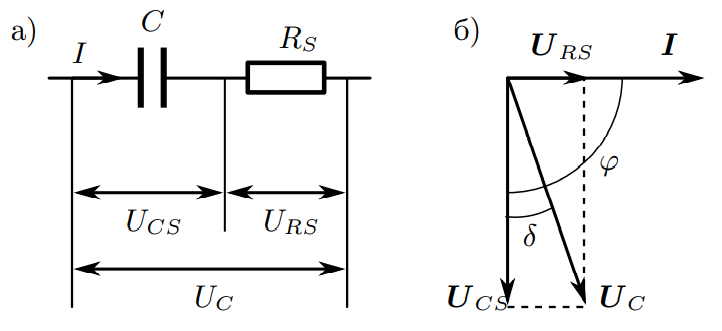
\includegraphics[width=0.7\textwidth]{eqCircuit.png}
    \caption{Последовательная эквивалентная схема конденсатора с потерями}
    \label{fig:eqCircuit}
\end{figure}

Для оценки возможного вклада активных потерь в конденсаторах в общий импеданс контура воспользуемся представлением конденсатора с ёмкостью $C$ последовательной эквивалентной схемой, показанной на рис. \ref{fig:eqCircuit}а. На этой схеме $R_S$~-— так называемое эквивалентное последовательное сопротивление (ЭПС), обусловленное, главным образом, электрическим сопротивлением материала обкладок и выводов конденсатора и контактов между ними, а также потерями в диэлектрике. Из эквивалентной схемы и векторной диаграммы к ней (рис. \ref{fig:eqCircuit}б) видно, что активные потери в конденсаторе, пропорциональные косинусу угла $\varphi$ сдвига фаз между током и напряжением на ёмкости, убывают с ростом $\varphi$ и соответственно с уменьшением угла $\delta = \pi/2 - \varphi$. Потери в конденсаторе принято характеризовать величиной $\tg \delta$, обычно приводимой в документации к изделию. Из рис. \ref{fig:eqCircuit} и закона Ома получаем выражение для ЭПС на циклической частоте $\omega = 2\pi\nu$ в виде

\begin{equation} \label{eq:EPS}
    R_S = \frac{U_{RS}}{I} = \frac{U_{RS}}{\omega CU_{CS}} = \frac{\tg \delta}{\omega C}. 
\end{equation}

Конденсаторы магазина ёмкостей экспериментальной установки в интересующем нас диапазоне частот имеют $\tg \delta < 10^{-3}$, что является очень хорошим (низким) показателем для конденсаторов с твёрдым диэлектриком.

\subsection{Свойства колебательного контура}

В колебательный контур, используемый в данной работе, добавлен резистор с сопротивлением $R$ для уменьшения добротности и упрощения получения АЧХ и АФХ. Таким, суммарное активное сопротивление контура принимается равным

\begin{equation}
    R_\Sigma = R + R_L + R_S.
\end{equation}

Добротность контура тем не менее остаётся достаточно высокой, чтобы можно было пользоваться следующими формулами:

\begin{equation} \label{eq:Q}
    Q = \frac{\rho}{R_\Sigma} = \frac{\omega_0L}{R_\Sigma} = \frac{1}{\omega_0 R\Sigma C} \gg 1.
\end{equation}

Для теоретического расчёта параметров контура используется метод комплексных амплитуд. Импеданс последовательного контура определяется по формуле:

\begin{equation}\label{импеданс}
	Z = R_\Sigma +i(\omega L - \frac{1}{\omega C}),
\end{equation}

где, $\omega_0$~-- резонансная частота контура, при которой импеданс~-- действительный. При условии, что $ | \Delta \omega | \ll \omega_0 $, формулы резонансных значений тока и напряжения имеют вид:

\begin{equation}\label{eq:Ires}
    I = \frac{E}{R_\Sigma}\cdot\frac{\cos(\omega t - \varphi_I)}{\sqrt{1+(\tau \Delta \omega )^2}}, 
\end{equation}

\begin{equation}\label{eq:Ures}
    U_C = E Q \frac{\omega_0}{\omega}\cdot\frac{\cos(\omega t - \varphi_C)}{\sqrt{1+\tau \Delta \omega )^2}},
\end{equation}

где

\begin{equation*}
	\varphi_I = -\arctg (\tau \Delta \omega ), 
\end{equation*}

\begin{equation}\label{phi_c}
	\varphi_C = -\frac{\pi}{2} + \delta - \arctg (\tau \Delta \varphi ).
\end{equation}

Здесь $ \tau = 2 Q / \omega_0 $~-- время затухания колебаний. Основные особенности резонанса в последовательном контуре, называемого также резонансом напряжений, из-за увеличения в $Q$ раз напряжений на ёмкости $U_C$ и индуктивности $U_L$ по отношению к внешнему напряжению $E$, следуют из анализа формул \eqref{eq:Ires}--\eqref{eq:Ures}. 

При отклонении $\Delta\omega$ частоты от резонансной таком, что выполнено условие 

\begin{equation}\label{eq:tomega}
   \tau\Delta\omega = \pm1, 
\end{equation}

амплитуда тока $I$, как видно из \eqref{eq:Ires}, уменьшается относительно резонансной в $\sqrt{2}$ раз, а фаза изменяется на $\pm\pi/4$. В этих же точках, если не учитывать поправки порядка $Q^{-1}$, происходят аналогичные изменения амплитуды $U_C$ и фазы $\varphi_C$. Величина $\delta\omega = 2|\Delta\omega| = 2/\tau$~-- ширина резонансной кривой на уровне $U_C(\omega_0)/\sqrt{2}$. По ней можно найти добротность контура: 

\begin{equation}\label{eq:Q2}
    Q = \frac{\omega_0}{\delta\omega}.
\end{equation}

\subsection{Экспериментальная установка}

Схема экспериментального стенда показана на рис. \ref{fig:setup}. Синусоидальный сигнал от генератора поступает на вход управляемого напряжением источника напряжения, собранного на операционном усилителе, питание которого осуществляется встроенным блоком-выпрямителем от сети $\sim 220 В$ (цепь питания на схеме не показана). Источник напряжения (источник с нулевым внутренним сопротивлением) обеспечивает с высокой точностью постоянство амплитуды сигнала на меняющейся по величине нагрузке~-- последовательном колебательном контуре, изображённом на рис. \ref{fig:setup} в виде эквивалентной схемы.

\begin{figure}[h]
    \centering
    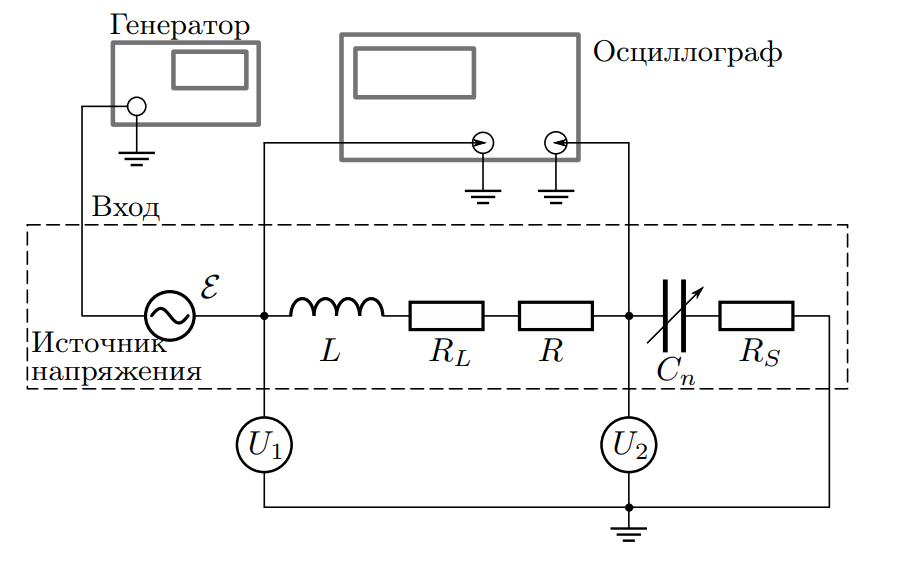
\includegraphics[scale=0.8]{setup.png}
    \caption{Схема установки для наблюдения резонанса напряжений}
    \label{fig:setup}
\end{figure}

Источник напряжения, колебательный контур и блок питания заключены в отдельный корпус, отмеченный на рисунке штриховой линией. На корпусе имеются коаксиальные разъёмы <<Вход>>, <<$U_1$>> и <<$U_2$>>, а также переключатель магазина ёмкостей $C_n$ с указателем номера $n = 1, 2,\dots 7$. Величины ёмкостей $C_n$ указаны на установке. Напряжение $E$ на контуре через разъём <<$U_1$>> попадает одновременно на канал 1 осциллографа и вход 1-го цифрового вольтметра. Напряжение на
конденсаторе $U_C$ подаётся через разъём <<$U_2$>> одновременно на канал 2
осциллографа и вход 2-го цифрового вольтметра.

\section{Оборудование и инструментальные погрешности}

\textbf{В работе используются:} генератор сигналов, источник напряжения,
нагрузкой которого является последовательный колебательный контур с
переменной ёмкостью, двухканальный осциллограф, цифровые вольтметры.

\textbf{Инструментальные погрешности:}
\begin{itemize}
    \item \textbf{Цифровые вольтметры:} $\delta_U = 1\%$;
    \item \textbf{Частотометр генератора:} $\delta_{f} = 0,1\%$;
    \item \textbf{Осциллограф:} $\delta_\varphi = 5\%$.
\end{itemize}

\section{Результаты измерений и обработка экспериментальных данных}

\begin{table}[h]
    \centering
    \begin{tabular}{|c|c|c|c|c|c|c|c|c|c|c|} \hline
        $C_n$, нФ & $f_{0n}$, кГц & $U_C$, B & $E$, B & $L$, мкГн & $Q$ & $\rho$, Ом & $R_\Sigma$, Ом & $R_{S_\text{max}}$, Ом & $R_L$, Ом & $I$, мА \\ \hline  
        25   & 27,9 & 2,04 & 0,148 & 1302 & 13,8 & 228,2 & 16,5 & 0,228 & 12,8 &  8,96 \\ \hline 
        33,2 & 26,7 & 2,87 & 0,148 & 1070 & 19,4 & 179,5 &  9,3 & 0,179 & 5,62 & 16,00 \\ \hline
        47,5 & 23,3 & 2,91 & 0,148 &  982 & 19,6 & 143,8 &  7,3 & 0,143 & 3,74 & 20,24 \\ \hline
        57,2 & 21,3 & 2,62 & 0,148 &  976 & 17,7 & 130,6 &  7,4 & 0,130 & 3,81 & 20,06 \\ \hline
        67,4 & 19,5 & 2,50 & 0,148 &  988 & 16,9 & 121,1 &  7,2 & 0,121 & 3,60 & 20,66 \\ \hline
        82,1 & 17,7 & 2,30 & 0,148 &  984 & 15,5 & 109,5 &  7,0 & 0,110 & 3,49 & 21.04 \\ \hline
        99,6 & 16,1 & 2,12 & 0,148 &  981 & 14,3 &  99,3 &  6,9 & 0,099 & 3,38 & 21,38 \\
        \hline
        \multicolumn{4}{|c|}{Среднее значение:} & 982 & & & & & 3,60 & \\ \hline
        \multicolumn{4}{|c|}{Погрешность:} &  12 & & & & & 0,24 & \\ \hline
    \end{tabular}
    \caption{Результаты измерения характеристик колебательного контура при разных значениях ёмкости}
    \label{tab:results}
\end{table}

В таблице представлены результаты измерения характеристик колебательного контура при разных значениях ёмкости магазина. Результаты первого измерения достаточно сильно отклоняются от средних, так как соответствующее значение добротности получается достаточно небольшим. 

На рис. \ref{graph:AFC1}, \ref{graph:AFC2}, \ref{graph:PFC2} представлены амплитудно-фазовая, относительная амплитудно-частотная и фазово-частотная характеристики для значений $C = C_1$ и $C = C_7$ ёмкости магазина. На рис. \ref{graph:AFC2} также отмечен уровень $1/\sqrt{2}$. По графику определено, что в обоих случаях полуширина амплитудно-частотной характеристики равна $\delta\omega =( 0,07\pm0,01)\omega_0 $. Отсюда получено значение добротности $Q = 14,3\pm1,2$.
 
\begin{figure}[h] \label{graph:AFC1}
\begin{center}
\begin{tikzpicture}
    \begin{axis}[
    xlabel={$f_{0n}$, кГц},
    ylabel={$U_C$, В},
    legend pos=north east,
    xmajorgrids=true,
    ymajorgrids=true,
    grid style=dashed,
    xmin = 0,
    ymin = 0,
    xmax = 40,
    ymax = 2
    ]
    \addplot[color=blue, mark=o] coordinates{
    (16.1, 0.22)
    (17.5, 0.24)
    (19.0, 0.27)
    (20.5, 0.31)
    (21.5, 0.35)
    (22.9, 0.43)
    (24.2, 0.59)
    (26.0, 0.96)
    (28.9, 1.45)
    (30.0, 0.90)
    (31.0, 0.61)
    (32.0, 0.47)
    (33.0, 0.37)
    (34.3, 0.29)
    (36.0, 0.22)
    (37.7, 0.18)
    };
    \addplot[color=red, mark=o] coordinates{
    (11.5, 0.30)
    (12.4, 0.35)
    (13.5, 0.47)
    (14.2, 0.62)
    (14.7, 0.79)
    (15.3, 1.18)
    (15.7, 1.78)
    (16.6, 1.51)
    (17.2, 0.94)
    (18.0, 0.59)
    (19.0, 0.38)
    (20.3, 0.26)
    (21.5, 0.19)
    (23.1, 0.14)
    (25.3, 0.10)
    };
    \legend{$n = 1$, $n = 7$}
    \end{axis}
\end{tikzpicture}
\caption{Амплитудно-частотные характеристики при $C = C_1$ и $C = C_7$}
\end{center}
\end{figure}

\begin{figure}[h] \label{graph:AFC2}
\begin{center}
\begin{tikzpicture}
    \begin{axis}[
    xlabel={$f_{0n}/f_0$},
    ylabel={$U_C/U_C(f_0)$},
    legend pos=north east,
    xmajorgrids=true,
    ymajorgrids=true,
    grid style=dashed,
    xmin = 0,
    ymin = 0,
    xmax = 2,
    ymax = 1.2
    ]
    \addplot[color=blue, mark=o] coordinates{
    (0.56, 0.15)
    (0.61, 0.17)
    (0.66, 0.19)
    (0.71, 0.22)
    (0.74, 0.24)
    (0.79, 0.30)
    (0.84, 0.41)
    (0.90, 0.66)
    (1.00, 1.00)
    (1.04, 0.62)
    (1.07, 0.42)
    (1.11, 0.32)
    (1.14, 0.26)
    (1.19, 0.20)
    (1.25, 0.15)
    (1.30, 0.12)
    };
    \addplot[color=red, mark=o] coordinates{
    (0.73, 0.17)
    (0.79, 0.20)
    (0.86, 0.26)
    (0.90, 0.35)
    (0.94, 0.44)
    (0.97, 0.66)
    (1.00, 1.00)
    (1.06, 0.85)
    (1.10, 0.53)
    (1.15, 0.33)
    (1.21, 0.22)
    (1.29, 0.15)
    (1.37, 0.11)
    (1.47, 0.08)
    (1.61, 0.06)
    };
    \legend{$n = 1$, $n = 7$}
    \addplot[color=orange]{0.714};
    \end{axis}
\end{tikzpicture}
\caption{Относительные амплитудно-частотные характеристики при $C = C_1$ и $C = C_7$}
\end{center}
\end{figure}

\begin{figure}[h] \label{graph:PFC2}
\begin{center}
\begin{tikzpicture}
    \begin{axis}[
    xlabel={$f_{0n}$, кГц},
    ylabel={$\varphi_C$},
    legend pos=north east,
    xmajorgrids=true,
    ymajorgrids=true,
    grid style=dashed,
    xmin = 0,
    ymin = 0,
    xmax = 40,
    ymax = 1.1
    ]
    \addplot[color=blue, mark=o] coordinates{
    (16.1, 1)
    (17.5, 1)
    (19.0, 1)
    (20.5, 0.96)
    (21.5, 0.96)
    (22.9, 0.95)
    (24.2, 0.93)
    (26.0, 0.86)
    (28.9, 0.26)
    (30.0, 0.15)
    (31.0, 0.13)
    (32.0, 0.10)
    (33.0, 0.07)
    (34.3, 0.05)
    (36.0, 0.04)
    (37.7, 0.02)
    };
    \addplot[color=red, mark=o] coordinates{
    (11.5, 1)
    (12.4, 0.98)
    (13.5, 0.96)
    (14.2, 0.93)
    (14.7, 0.91)
    (15.3, 0.84)
    (15.7, 0.71)
    (16.6, 0.27)
    (17.2, 0.18)
    (18.0, 0.09)
    (19.0, 0.06)
    (20.3, 0.04)
    (21.5, 0.03)
    (23.1, 0.02)
    (25.3, 0.015)
    };
    \legend{$n = 1$, $n = 7$}
    \end{axis}
\end{tikzpicture}
\caption{Фазово-частотные характеристики при $C = C_1$ и $C = C_7$}
\end{center}
\end{figure}

\section{Обсуждение результатов и выводы}

Измеренные при разных значениях ёмкости значения параметров системы, от неё не зависящих, совпадают качественно, но слегка отличаются в зависимости от значения ёмкости.

Полученные разными методами средние значения добротности~-- $Q_\text{эксп} = 16,7\pm1,1$ и $Q_\text{АЧХ} = 14,3\pm1,2$~-- совпадают в пределах нескольких стандартных отклонений, но тем не менее отличны друг от друга. Связано это с недостаточной точностью определения добротности как первым, так и вторым способом. Причиной этому являются как инструментальные погрешности и дефекты установки, так и недостаточно высокое значение добротности ($\sim10^1$), из чего следует меньшая точность применённых в работе формул.

Таким образом, нам удалось пронаблюдать явление резонанса напряжений в последовательном колебательном контуре и измерить качественные характеристики контура в резонансе и вблизи него. Применённые методы позволяют оценить параметры катушки и других элементов цепи по порядку величины, однако они не дают возможности с точностью получить реальные характеристики элементов. Использованные в работе методы определения добротности будут более применимы для установок с меньшим или отсутствующим добавочным сопротивлением.

\end{document}